\documentclass[xcolor=dvipsnames, 9pt]{beamer} % dvipsnames gives more built-in colors

% theme and color settings
\usetheme{Madrid}
\useoutertheme[hideothersubsections, left, height=0pt]{sidebar}
\useinnertheme{circles}

\definecolor{insead_dark}{RGB}{0,110,91} 
\definecolor{insead_light}{RGB}{160,206,103}
\definecolor{fade}{HTML}{C1C7D0}
\definecolor{light_red}{HTML}{DCBCBC}
\definecolor{mid_red}{HTML}{B97C7C}
\definecolor{dark_red}{HTML}{8F2727}

\usecolortheme[named=insead_dark]{structure}
\usefonttheme[onlymath]{serif}

% some packages 
\usepackage{xcolor}
\usepackage{graphicx} 
\usepackage{booktabs} 
\usepackage{multicol}
\usepackage{tikz}
\usepackage{setspace}
\usepackage{tcolorbox}
\usepackage{colortbl}

%frontmatter
\title[Session 1 (Basics)]{\normalsize{MBA Business Foundations, \\Quantitative Methods: \\Session One}}
\author[Boris Babic, INSEAD]{Boris Babic, \\Assistant Professor of Decision Sciences}
\institute[]{}
\date{}

%\beamerdefaultoverlayspecification{<+->}

\begin{document}

\setbeamertemplate{sidebar left}{}
\begin{frame}
\titlepage
\vspace{-5em}
\begin{center}

\includegraphics[scale=0.4]{/Users/borisbabic/_INSEAD_teaching/_business_foundations/_syllabus/insead_logo.png}
\end{center}
\end{frame}

\begin{frame}
\frametitle{About me}
\begin{flushright}
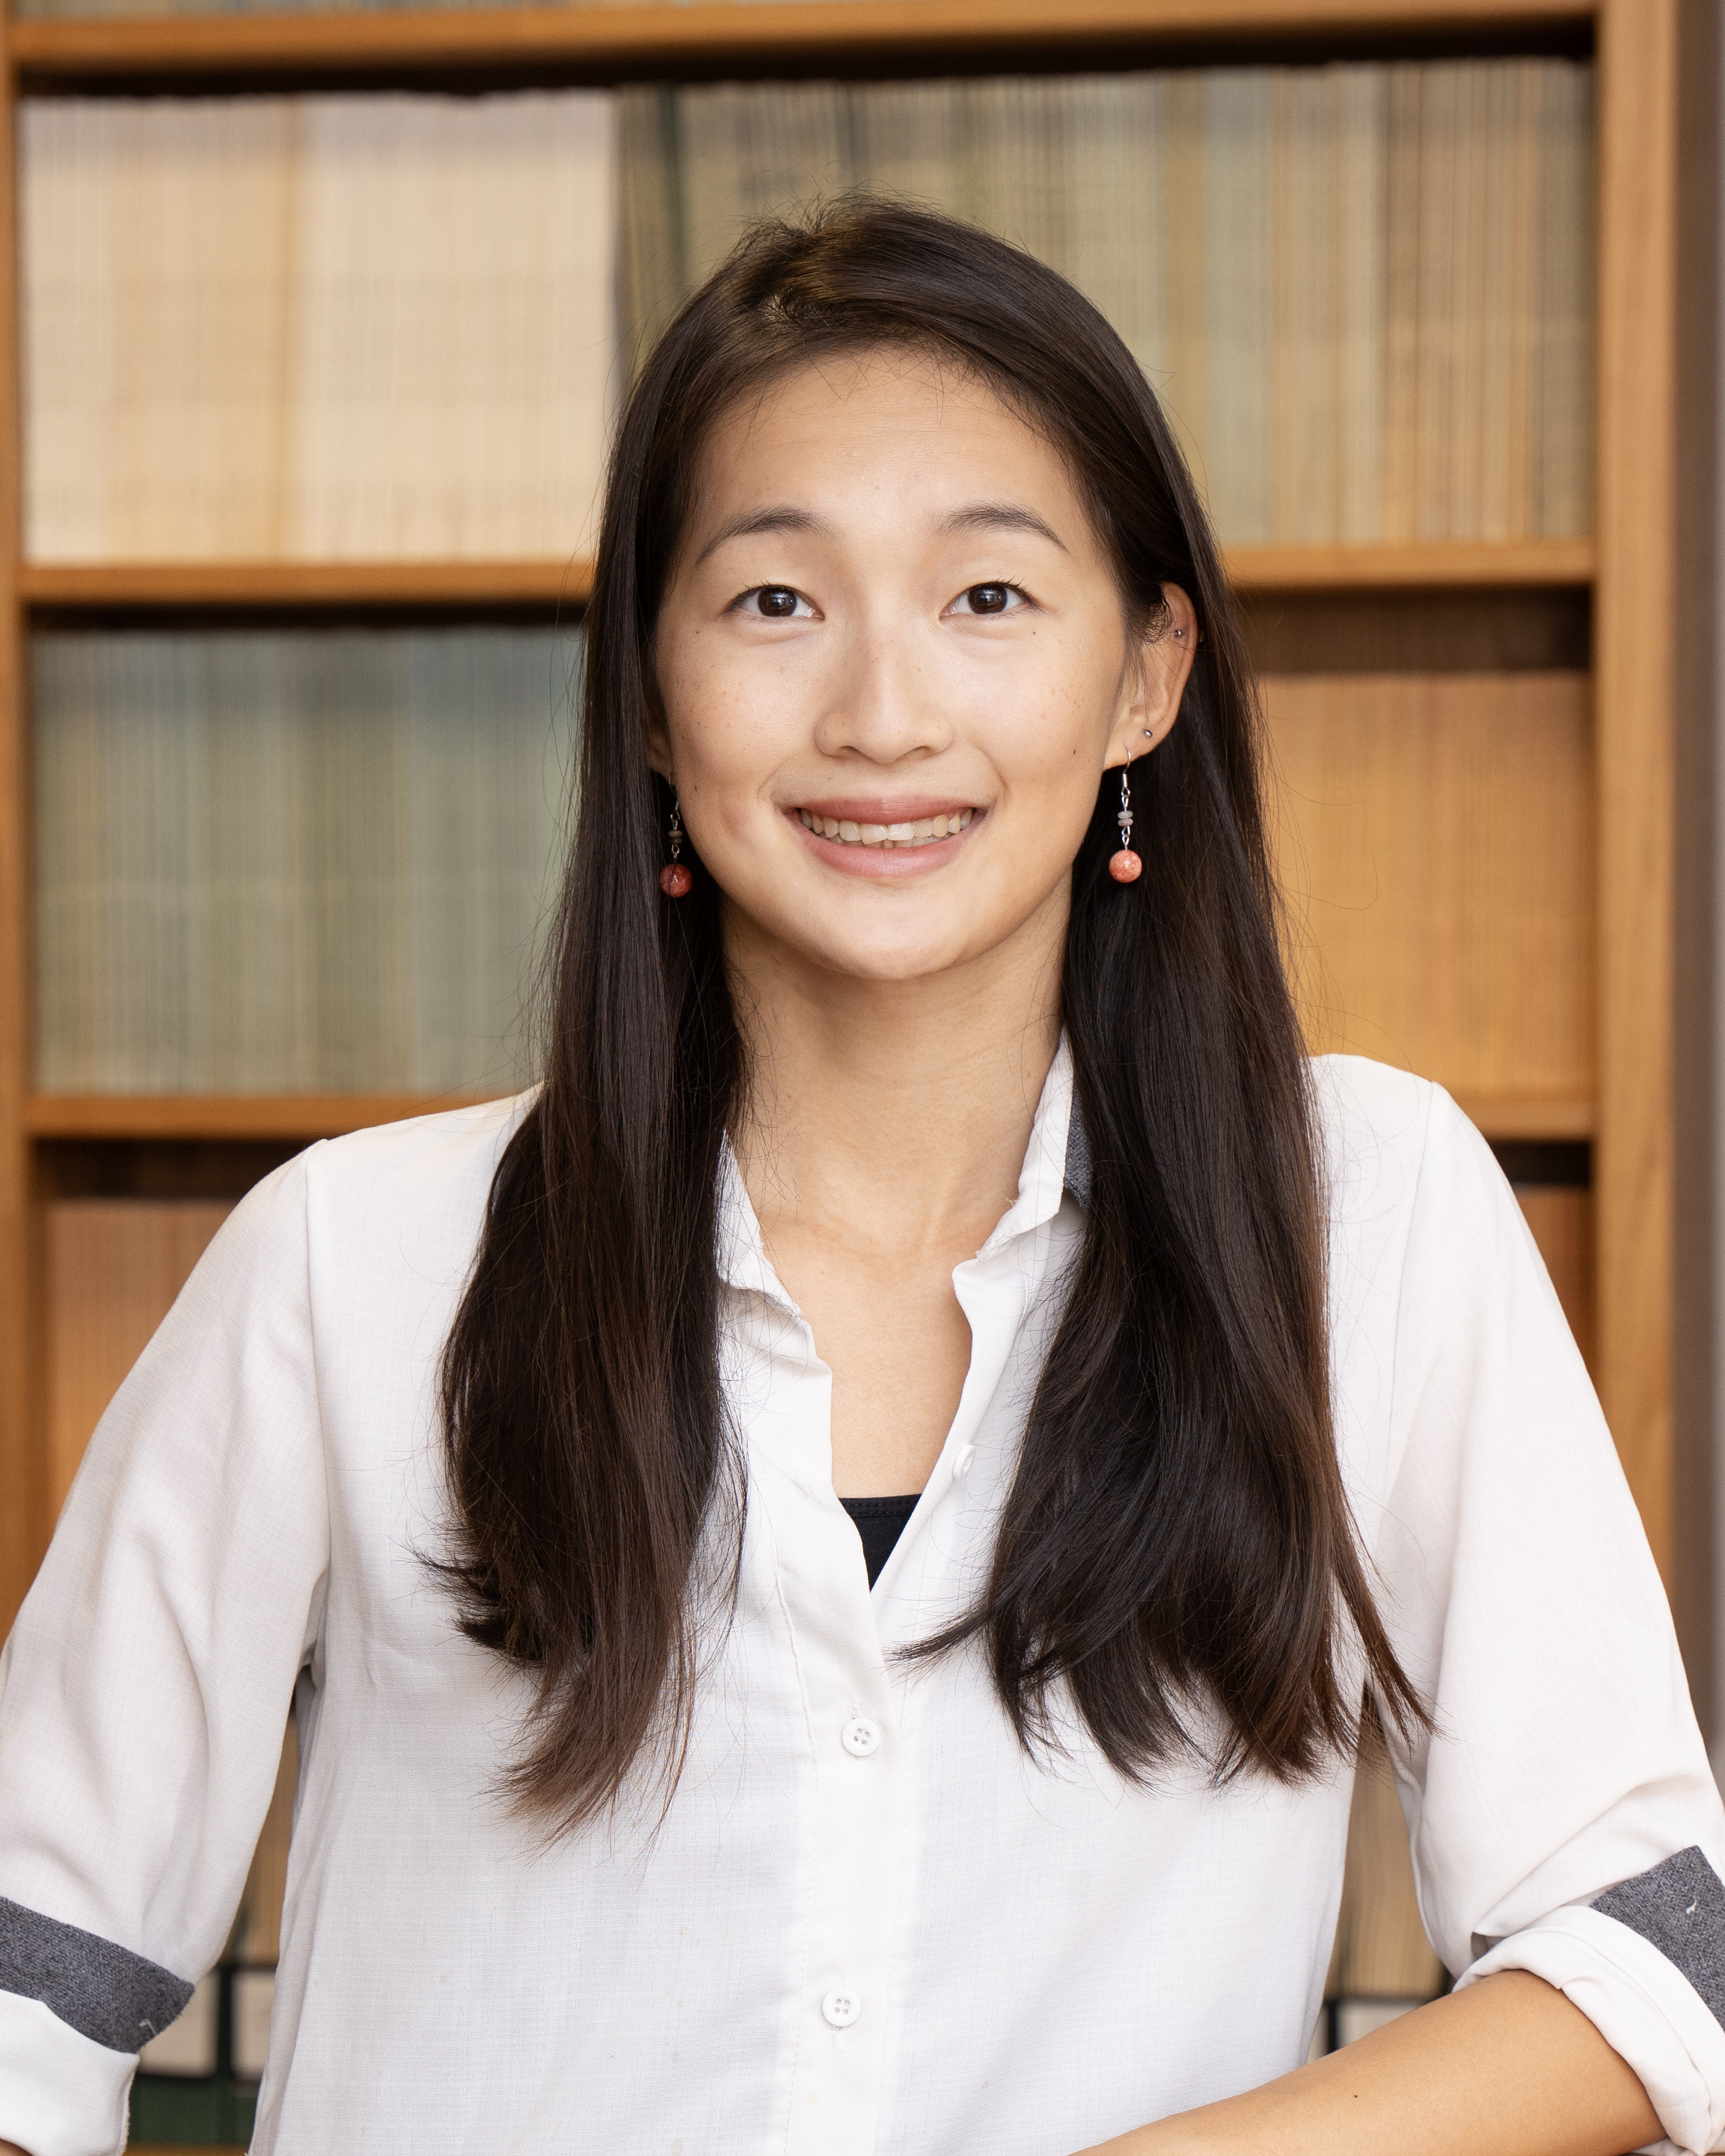
\includegraphics[scale=0.3]{profile.png}
\end{flushright}
\vspace{-11em}
\begin{itemize}
	\setlength\itemsep{1em}
\item Joined INSEAD June 2019
\item Fist time teaching MBA's, have taught PhDs/JDs.
\item Postdoc, California Institute of Technology
\item PhD/MS, University of Michigan (Ann Arbor) 
\item[] \includegraphics[scale=0.25]{goblue.png}
\item JD, Harvard Law School 
\item Former trial lawyer 
\item Research is in Bayesian statistics and ethics of AI/ML 
\item Teach MBA Management Decision Making! \\ (See you there!!)
\end{itemize}
\end{frame}
%\item[] \includegraphics[scale=0.2]{caltech.png} %\includegraphics[scale=0.25]{jpl.png}


\begin{frame}
\frametitle{About your classmates}

\begin{center}
\includegraphics[scale=0.4]{demographics.png}
\end{center}

\begin{center}
\includegraphics[scale=0.4]{demographics2.png}
\end{center}

\end{frame}


\begin{frame}
\frametitle{Course structure}
\begin{itemize}
	\itemsep\setlength{1em}
\item Two overarching features: (a) mixed backgrounds, (b) packed schedule!
\item Structure: \textcolor{red}{follow a clear fixed path} + bonus adventures for the curious
\item[] Ex: I will post all my workflow (LaTeX, Python, Mathematica notebooks)
\item Focus on exercises/learning by doing!
\item 5 classes, focus on applications to management and finance
\item Readings before each lecture
\item Exercises after each lecture (due the following lecture)
\item[] Will not be graded, but I will post solutions
\item Study period in the afternoon, I will be around (Office 543)
\item \textcolor{red}{If anything is unclear, come talk to me!}
\item Website: \textcolor{red}{\href{borisbabic.com/teaching/inseadqm/home}{borisbabic.com/teaching/inseadqm/home}}
\end{itemize}
\end{frame}

\begin{frame}
\frametitle{Content}
\begin{small}
\begin{tabular}{ll}
\textcolor{insead_dark}{Basics} & \begin{tabular}[c]{@{}l@{}}Functions\\ Linear\\ Inverse\\ Two equations\\ Quadratic\end{tabular} \vspace{0.25em} \\ 

\textcolor{insead_dark}{Exponents}   & \begin{tabular}[c]{@{}l@{} }\hline \\ Exponents\\ Application: interest rates\\ Exponential functions\\ Logarithmic functions\end{tabular} \vspace{0.25em} \\

\textcolor{insead_dark}{Logarithms} & \begin{tabular}[c]{@{}l@{}} \hline \\ Logarithmic functions\\ Logarithmic and exponential equations \\ Case: pricing\\ Derivatives \end{tabular}   \vspace{0.25em}  \\

\textcolor{insead_dark}{Derivatives}  & \begin{tabular}[c]{@{}l@{}} \hline \\ Optimal decisions\\ Case: production\\ Statistics\end{tabular}        \vspace{0.25em} \\

\textcolor{insead_dark}{Uncertainty}    & \begin{tabular}[c]{@{}l@{}} \hline \\ Probability \& statistics\\ Normal distribution \end{tabular}     \vspace{0.25em} \\       
\end{tabular}
\end{small}
\end{frame}

\begin{frame}
\frametitle{Today}
\begin{small}
\begin{tabular}{ll}
\textcolor{insead_dark}{Basics} & \begin{tabular}[c]{@{}l@{}}Functions\\ Linear\\ Inverse\\ Two equations\\ Quadratic\end{tabular} \vspace{0.25em} \\ 

\textcolor{fade}{Exponents}   & \begin{tabular}[c]{@{}l@{} }\arrayrulecolor{fade}\hline \\ \textcolor{fade}{ Exponents}\\ \textcolor{fade}{ Application: interest rates}\\ \textcolor{fade}{Exponential functions}\\ \textcolor{fade}{Logarithmic functions}\end{tabular} \vspace{0.25em} \\

\textcolor{fade}{Logarithms} & \begin{tabular}[c]{@{}l@{}} \arrayrulecolor{fade}\hline \\ \textcolor{fade}{Logarithmic functions}\\ \textcolor{fade}{Logarithmic and exponential equations} \\ \textcolor{fade}{Case: pricing}\\ \textcolor{fade}{Derivatives} \end{tabular}   \vspace{0.25em}  \\

\textcolor{fade}{Derivatives}  & \begin{tabular}[c]{@{}l@{}} \arrayrulecolor{fade}\hline \\ \textcolor{fade}{Optimal decisions}\\ \textcolor{fade}{Case: production}\\\textcolor{fade}{ Statistics}\end{tabular}        \vspace{0.25em} \\

\textcolor{fade}{Uncertainty}    & \begin{tabular}[c]{@{}l@{}} \arrayrulecolor{fade}\hline \\\textcolor{fade}{ Probability \& statistics}\\ \textcolor{fade}{Normal distribution }\end{tabular}     \vspace{0.25em} \\       
\end{tabular}
\end{small}
\end{frame}

\setbeamertemplate{sidebar left}[sidebar theme]
\section{Functions}

\begin{frame}
\frametitle{Constants vs. variables}

\begin{itemize}
\item[] Constant
	\begin{itemize}
		\item Definition: placeholder for a given or fixed value
		\item Notation: $a, b, c$
		\item Examples: 
		\begin{itemize}
		\item Maximum number of units that can be produced on a production line 
		\item Height of the Eiffel tower
		\end{itemize}
	\end{itemize}
\item[]	Variable
\begin{itemize}
		\item Definition: Placeholder for an unknown value 
		\item Notation: $x, y, z$
		\item Examples:  
		\begin{itemize}
		\item Number of units produced each day on a production line  
		\item Height of a student in this class 
		\end{itemize}
	\end{itemize}
\end{itemize}
\end{frame}

\begin{frame}
\frametitle{Continuous vs. discrete variables}

\begin{itemize}
\item[] Continuous
	\begin{itemize}
		\item Can take values within a range
		\item Examples: height, weight, etc. 
	\end{itemize}
\item[]	Discrete
\begin{itemize}
		\item Can take only certain values (typically whole numbers)
		\item Examples: number of children, number of defective products, number of weeks worked
	\end{itemize}
\end{itemize}
\end{frame}

\begin{frame}
\frametitle{Functions}
\begin{itemize}
\item A function is a type of map: 
\item[] \begin{equation*}
x \textrm{~(Input)} \longrightarrow \textcolor{dark_red}{f} \textrm{\textcolor{dark_red}{~(Function)}} \longrightarrow y = f(x) \textrm{(Output)}
\end{equation*}
\item Here we say $f$ maps $x$ to $y$. For example, the following function maps shapes to their associated colors. 
\vspace{-1em}
\begin{center}
\item[] \includegraphics[scale=0.35]{function_example.png}
\end{center}
\vspace{-1em}
\item Does it matter that no blue shape? That two red shapes? 
\item $x$ is the independent variable, $y$ is the dependent variable. 
\item $f$ is the operation done on $x$ to get $y$ -- the function, usually denoted $f, g, h$.
\end{itemize}
\end{frame}

\begin{frame}
\frametitle{Functions: examples}
\begin{itemize}
\item Eg: Let $f(x) = x + 2$. Then if $x = 3$, $y = f(x) = 5$. 
\item Eg: Amount of interest earned ($I$) depends on the length of time money is invested ($t$), given both money invested ($p$) and interest rate ($r$): 
\item[] $I = t \times p \times r$ 
\item[] $I = 10000 \times 0.04 t = 400t$. If $t = 5$ then $I = \$2,000$ \\
\item[] $y = f(t)$ 
\item Eg: Revenue of a firm ($R$) is a function of quantity
of product sold ($q$), given the price ($p$)
\item[] $R = \textrm{price} \times \textrm{quantity} \rightarrow R =  p \times q \rightarrow R = 5q $
\item[] $R = g(q)$ (why does $p$ not appear in the expression?)
\end{itemize}
\end{frame}

\begin{frame}
\frametitle{Graphs}
A convenient way to visualize functions: 

\hspace*{-0.5cm} \includegraphics[scale=0.4]{graph1.png}

Gives a visual representation of the relationship between two quantities
\end{frame}

\begin{frame}
\frametitle{Some examples of graphs}
Google searches for ``Manchester United" in Singapore as a function of time (previous 90 days)
\includegraphics[scale=0.26]{mufc.png}
\end{frame}

\begin{frame}
\frametitle{Some examples of graphs}
\includegraphics[scale=0.5]{pop_growth2.png}
\end{frame}


\section{Linear}

\begin{frame}
\frametitle{Linear functions}
Functions of a special form:

\hspace*{-0.6cm} \includegraphics[scale=0.3]{slope_intercept.png}
\hspace*{-0.4cm} \includegraphics[scale=0.3]{slope_int_chart.png}

\end{frame}

\begin{frame}
\frametitle{Linear functions}
How to plot a linear function $y = ax + b$? \\
\hspace*{-0.35cm} \includegraphics[scale=0.3]{find_points.png} 
\end{frame}

\begin{frame}
\frametitle{Example}
\begin{itemize}
		\item Ex: Let $ f(x) = 2x + 4$. Plot this graph.
		\item $(0, b) = \textcolor{dark_red}{(0, 4)}$
		\item $(-b/a, 0) = (-4/2, 0) = \textcolor{dark_red}{(-2, 0)}$
\item[] \begin{center} \hspace*{-0.35cm} \includegraphics[scale=0.5]{slope_int_eg.pdf} \end{center}
\end{itemize}
\end{frame}

\begin{frame}
\frametitle{Finding the linear form}

A grocery store owner starts her business with debts \$100,000. After operating for five years, she has accumulated a net profit of \$40,000. Write a linear rule for profit as a function of time. That is, write it in the form $$ y = ax + b$$ where $y$ is profit and $x$ is time. 

\end{frame}

\begin{frame}
\frametitle{Finding the linear form}

$$ y = -100000 + 28000x $$

\hspace*{-0.6cm} \includegraphics[scale=0.4]{graph2.png}
Linear functions are... 
\begin{itemize}
\item Easy to estimate 
\item Easy to analyze
\item Easy to interpret (and surprisingly general!)
\end{itemize}
\end{frame}

\begin{frame}
\frametitle{Finding the intersection of two lines}
\begin{itemize}
	\itemsep\setlength{1em}
		\item Example: Nuclear vs. fuel power plants 
		\item Suppose cost $C$ is a linear function of quantity $Q$, where $N$ stands for Nuclear and $F$ stands for Fuel.
		\item[] $C_N = 1000 + Q_N$
		\item[] $C_F = 100 + 3Q_F$
		\item Plot the two lines
		\item At what point do the two plants have the same cost?
\end{itemize}

\end{frame}

\begin{frame}
\frametitle{Finding the intersection of two lines}
\begin{center}
\includegraphics[scale=0.5]{intersection.png}
\end{center}
\end{frame}

\section{Inverse}

\begin{frame}
\frametitle{Inverse functions }
An inverse function is a different type of map: 
\begin{equation*}
x = f^{-1}(y) \textrm{~(Input)} \longleftarrow \textcolor{dark_red}{f^{-1}} \textrm{\textcolor{dark_red}{~(Inverse function)}} \longleftarrow y~\textrm{(Output)}
\end{equation*}
\begin{itemize}
\item Note that $f^{-1}(f(x)) = x$
\item Ex: if $f(x) = x^2$, what is $f^{-1}(x)$? \\
\item Ex: If $g(x) = x^3 + 3$, what is $g^{-1}(x)$?
\item Ex: if $h(x) = 7x^2 + 4$ what is $h^{-1}(x)$?
\item[\textcolor{insead_dark}{$\rightarrow$}] Answers:
\item $f^{-1}(x) = \sqrt{x}$
\item $g^{-1}(x) = \sqrt[3]{x -3}$
\item $h^{-1}(x) = \sqrt{\frac{x - 4}{7}}$
\end{itemize}
\end{frame}

\begin{frame}
\frametitle{Recipe}
\begin{enumerate}
\itemsep\setlength{1em}
\item Replace $f(x)$ with a $y$
\item Swap $x$ and $y$
\item Solve for $y$
\item Replace $y$ with $f^{-1}$
\item[] Example from above: 
\begin{align*}
g(x) = x^3 + 3 \tag{original function} \\
\leftrightarrow y = x^3 + 3 \tag{step 1} \\
\leftrightarrow x = y^3 + 3 \tag{step 2} \\
\leftrightarrow y = \sqrt[3]{x - 3} \tag{step 3} \\
\leftrightarrow g^{-1}(x) = \sqrt[3]{x - 3} \tag{step 4}
\end{align*}
\end{enumerate}

\end{frame}

\begin{frame}
\frametitle{Graphical relationship}
\vspace{-1.5cm}
$\sqrt{\textcolor{dark_red}{x^2}} = x$ 
\begin{flushright}
\hspace*{-0.6cm} \includegraphics[scale=0.35]{graph3.png}
\hspace*{2cm} \includegraphics[scale=0.3]{xcubed.png}
\end{flushright}
\vspace{-3cm}

$ \sqrt[3]{\textcolor{dark_red}{x^3 + 3} - 3} = x $
\end{frame}

\begin{frame}
\frametitle{Example from economics}
\hspace*{-0.25cm} \includegraphics[scale=0.3]{inv_demand.png}
\end{frame}

\section{Two Equations}

\begin{frame}
\frametitle{Systems of equations}
\begin{scriptsize}
\begin{tabular}{l|l|l}
 & By substitution & By elimination \\
Method & \begin{tabular}[c]{@{}l@{}} \\ Find $x$ in the first equation, \\ plug it into the second equation\end{tabular} & \begin{tabular}[c]{@{}l@{}} \\ Eliminate one unknown by \\ adding up the two equations \end{tabular} \\
Examples & \begin{tabular}[c]{@{}l@{}}\\ $3x - 2y = 16$ \\ $x + y = 2$\end{tabular} & \begin{tabular}[c]{@{}l@{}}\\ $x + y = 7$\\ $x - y = 1$\end{tabular}
\end{tabular}

\vspace{1em}
%\pause
\begin{itemize}
\item By substitution (left panel example): 
\begin{align*}
x = 2 - y 
&\rightarrow 3(2-y) - 2y = 16 \\
&\rightarrow 6 - 3y - 2y = 16 \\
&\rightarrow 6 - 5y = 16 \\
&\rightarrow 5y = -10 \\
&\rightarrow y = -2 \rightarrow x = 4
\end{align*}
\item By elimination (right panel example): $2x = 8 \rightarrow x = 4 \rightarrow y = 3$
\end{itemize}
\end{scriptsize}
\end{frame}

\begin{frame}
\frametitle{Examples }

\begin{itemize}
\item Ex 1:
\item[] $3x - y = 7$
\item[] $2x + 3y = 1$
\item Ex 2:
\item[] $5x + 4y = 1$
\item[] $3x - 6y = 2$
\item Solution 1: $x = 2, y = -1$
\item Solution 2: $x = 1/3, y = -1/6$
\end{itemize}

\end{frame}

\section{Quadratic}

\begin{frame}
\frametitle{Quadratic functions}
Another special type of function (a type of polynomial), of the form $$ \textcolor{dark_red}{a}x^2 + \textcolor{dark_red}{b}x + \textcolor{dark_red}{c} $$

\begin{itemize}
\item When $a = 0$ we recover a linear function.
\item When $ a \neq 0$, this is a nonlinear function. Its graph is a continuous curve called a parabola. 
\end{itemize}

\hspace*{-0.6cm} \includegraphics[scale=0.36]{graph4.png}
\hspace*{-0.6cm} \includegraphics[scale=0.36]{graph5.png}

\end{frame}

\begin{frame}
\frametitle{Quadratic equations}
\begin{itemize}
\item Solving quadratic function equal to $0$. 
\item Goal: $x$ such that $ax^2 + bx + c = 0$.
\item[] \hspace*{1cm} \includegraphics[scale=0.4]{quad_eq.png}
\item Corresponds to the intersection(s) of the curve with $f(x) = 0$ line.\\
\item Will there aways be solutions to this problem? \\
\item Depends on the value of $b^2 - 4ac$. 
\end{itemize}
\end{frame}

\begin{frame}
\frametitle{Quadratic equations}
\begin{itemize}
	\itemsep\setlength{1em}
\item In general, when $ax^2 + bx + c = 0$, the roots are:
\item[] $$ \textcolor{dark_red}{ x = \frac{-b \pm \sqrt{b^2 - 4ac} }{2a} }$$
\item If $b^2 - 4ac > 0$ then 2 roots
\item If $b^2 - 4ac = 0$ then 1 root
\item If $b^2 - 4ac < 0$ then no roots
\end{itemize}
\end{frame}


\begin{frame}
\frametitle{Exercises}

\begin{itemize}
	\itemsep\setlength{1em}
\item Ex 1: Solve $x^2 - x -2 = 0$
\item Ex 2: Solve $4x^2 - 12x + 9 = 0$
\item Ex 3: Solve $x^2 - 2x + 3 = 0$
\item Solution 1: $x = -1, x=2$
\item Solution 2: $x = 3/2$
\item Solution 3: No real solution
\end{itemize}
\end{frame}

\begin{frame}
\frametitle{Graphed solutions}
\begin{center}
\includegraphics[scale=0.5]{root_solutions.png}
\end{center}
\end{frame}

\begin{frame}
\frametitle{Application to market equilibrium}
\begin{itemize}
	%\itemsep\setlength{1em}
\item[] Suppose that supply, $S$, and demand, $D$, for a product are functions of the product price, $p$:
\item[] $S = p^2 + 10p + 10$
\item[] $D = 110 - 10p$
\item[] At what price will supply equal demand? 
\end{itemize}
\end{frame}

\begin{frame}

\frametitle{Application to market equilibrium}
\begin{align*}
& ~ p^2 + 10p + 10 = 110 - 10p \\
\leftrightarrow & ~ p^2 + 20p - 100 = 0 \\ 
\rightarrow & ~ p = \frac{-20 \pm \sqrt{20^2 - 4\times 1 \times -100 }}{2 \times 1} \\
& ~ p \approx 4.24 
\end{align*}
\hspace*{1cm} \includegraphics[scale=0.5]{quad_eq2.png}
\end{frame}

\begin{frame}
\frametitle{Profit-break even analysis}
The demand function for a good is given as $Q = 65 - 5p$, where $Q$ is quantity and $p$ is price. Fixed costs are $\$30$ and each unit produced costs an additional $\$2$.

\vspace{1em}

Write down the equations for total revenue and total costs as a function of $Q$.

\vspace{1em}

Find the break-even point(s). 
\end{frame}

\begin{frame}
\frametitle{Application to market equilibrium}
\hspace{0.5cm} \includegraphics[scale=0.4]{quad_eq3.png}
\end{frame}

\begin{frame}
\frametitle{Resources}
\begin{small}
\begin{itemize}
\item Paul's Notes (for excellent notes): \href{http://tutorial.math.lamar.edu/Extras/AlgebraTrigReview/AlgebraTrigIntro.aspx}{\textcolor{dark_red}{http://tutorial.math.lamar.edu/Extras/AlgebraTrigReview/AlgebraTrigIntro.aspx}}
\item Khan Academy Algebra (for additional lectures): \href{https://www.khanacademy.org/math/algebra}{\textcolor{dark_red}{https://www.khanacademy.org/math/algebra}}
\item WolframAlpha (for computing answers): \href{https://www.wolframalpha.com/}{\textcolor{dark_red}{https://www.wolframalpha.com/}}
\item Math Stack Exchange (for questions): \href{https://math.stackexchange.com/}{\textcolor{red}{https://math.stackexchange.com/}}
\end{itemize}
\end{small}
\end{frame}

\begin{frame}
\frametitle{Today}
\begin{small}
\begin{tabular}{ll}
\textcolor{insead_dark}{Basics} & \begin{tabular}[c]{@{}l@{}}Functions\\ Linear\\ Inverse\\ Two equations\\ Quadratic\end{tabular} \vspace{0.25em} \\ 

\textcolor{fade}{Exponents}   & \begin{tabular}[c]{@{}l@{} }\arrayrulecolor{fade}\hline \\ \textcolor{fade}{ Exponents}\\ \textcolor{fade}{ Application: interest rates}\\ \textcolor{fade}{Exponential functions}\\ \textcolor{fade}{Logarithmic functions}\end{tabular} \vspace{0.25em} \\

\textcolor{fade}{Logarithms} & \begin{tabular}[c]{@{}l@{}} \arrayrulecolor{fade}\hline \\ \textcolor{fade}{Logarithmic functions}\\ \textcolor{fade}{Logarithmic and exponential equations} \\ \textcolor{fade}{Case: pricing}\\ \textcolor{fade}{Derivatives} \end{tabular}   \vspace{0.25em}  \\

\textcolor{fade}{Derivatives}  & \begin{tabular}[c]{@{}l@{}} \arrayrulecolor{fade}\hline \\ \textcolor{fade}{Optimal decisions}\\ \textcolor{fade}{Case: production}\\\textcolor{fade}{ Statistics}\end{tabular}        \vspace{0.25em} \\

\textcolor{fade}{Uncertainty}    & \begin{tabular}[c]{@{}l@{}} \arrayrulecolor{fade}\hline \\\textcolor{fade}{ Probability \& statistics}\\ \textcolor{fade}{Normal distribution }\end{tabular}     \vspace{0.25em} \\       
\end{tabular}
\end{small}
\end{frame}

%endnotes
	{\setbeamercolor{background canvas}{bg=insead_dark}
    \begin{frame}[plain]
    \begin{tikzpicture}[remember picture,overlay]
    \node[at=(current page.center)] {
    \includegraphics[keepaspectratio,
    width=\paperwidth,
    height=\paperheight]{/Users/borisbabic/_INSEAD_teaching/_business_foundations/_syllabus/end_slide.png}};
    \end{tikzpicture}
    \end{frame}}
\end{document}